
% This LaTeX was auto-generated from an M-file by MATLAB.
% To make changes, update the M-file and republish this document.

\documentclass[11pt]{article}
\usepackage{amsmath,amsfonts,amsthm,amssymb}
\usepackage{fullpage,fancyhdr}
\usepackage[pdftex]{graphicx}
\usepackage[usenames,dvipsnames]{color}
\usepackage{listings}
\usepackage{courier}
\usepackage{ifthen}
\usepackage{setspace}
\usepackage{lastpage}
\usepackage{extramarks}
\usepackage{chngpage}
\usepackage{soul}
\usepackage{graphicx,float,wrapfig}
\usepackage{epstopdf}
\usepackage{geometry}
\usepackage{pdfcolmk}
\usepackage{hyperref}
\DeclareGraphicsRule{.tif}{png}{.png}{`convert #1 `dirname #1`/`basename #1 .tif`.png}

\definecolor{lightgray}{gray}{0.5}
\definecolor{darkgray}{gray}{0.3}
\definecolor{MyDarkGreen}{rgb}{0.0,0.4,0.0}

\topmargin=-0.45in      %
\evensidemargin=0in     %
\oddsidemargin=0in      %
\textwidth=6.5in        %
\textheight=9.0in       %
\headsep=0.25in         %

\pagestyle{fancyplain}

% For faster processing, load Matlab syntax for listings
\lstloadlanguages{Matlab}%
\lstset{language=Matlab,
        frame=single,
        basicstyle=\ttfamily,
        keywordstyle=[1]\color{Blue}\bf,
        keywordstyle=[2]\color{Purple},
        keywordstyle=[3]\color{Blue}\underbar,
        identifierstyle=,
        commentstyle=\usefont{T1}{pcr}{m}{sl}\color{MyDarkGreen}\small,
        stringstyle=\color{Purple},
        showstringspaces=false,
        tabsize=5,
        % Put standard MATLAB functions not included in the default
        % language here
        morekeywords={xlim,ylim,var,alpha,factorial,poissrnd,normpdf,normcdf},
        % Put MATLAB function parameters here
        morekeywords=[2]{on, off, interp},
        % Put user defined functions here
        morekeywords=[3]{FindESS},
        morecomment=[l][\color{Blue}]{...},
        numbers=left,
        firstnumber=1,
        numberstyle=\tiny\color{Blue},
        stepnumber=5
        }

 
\fancyhf{}
 
\lhead{\fancyplain{}{Michael Carroll}}
\chead{\fancyplain{}{ELEC6410 - DSP}}
\rhead{\fancyplain{}{\today}}
\rfoot{\fancyplain{}{\thepage\ of \pageref{LastPage}}}



    \title{ELEC6410 Project 3\\
    {\large Answers to Digital Signal Processing Project \#3}}
    \author{Michael J. Carroll}


\begin{document}
\maketitle


           
        \subsection*{Question 1}
    Examine a sampled waveform
% end of cell

    
           
        \subsection*{Part A}
    Sample the waveform $x(t) = 3\cos{3000\pi t} + \cos{800\pi t}$ at a sampling frequency of 16 kHz for one second:Since the signal is sampled at greater than the Nyquist rate, it may be treated as a continuous signal.
\begin{lstlisting}[language=matlab]
t = [0:1/16000:1];
xc = 3*cos(3000*pi*t) + cos(800*pi*t);
\end{lstlisting}

% end of cell

    
           
        \subsection*{Part B}
    Plot the first 100 points of the signal with an appropriately labeled t axis.Plot is used for the case of a continuous signal in Figure ~\ref{fig:figure1}.
\begin{lstlisting}[language=matlab]
figure(1);
plot(t(1:100),xc(1:100));
xlabel('Time in Seconds'); ylabel('Amplitude');
title('First 100 Points of Waveform xc');
\end{lstlisting}

\begin{figure}[here]
	\begin{center}
		\includegraphics [width=4in]{Project3_01.eps}
		\caption{}
		\label{fig:}
	\end{center}
\end{figure}

% end of cell

    
           
        \subsection*{Part C}
    Plot the Fourier-transform magnitude of x(t).
\begin{lstlisting}[language=matlab]
figure(2);
plot([-8000:7999],fftshift(abs(fft(xc(1:2*8000)))));
xlabel('Normalized Frequency (\times 2\pi to give rad/s)');
title('Fourier-transform magnitude of waveform xc');
\end{lstlisting}

\begin{figure}[here]
	\begin{center}
		\includegraphics [width=4in]{Project3_02.eps}
		\caption{}
		\label{fig:}
	\end{center}
\end{figure}

% end of cell

    
           
        \subsection*{Part D}
    Explain how this graph corresponds to the actual Fourier transform of x(t).The plot of the Fourier transform in Figure ~\ref{fig:figure2}.  The important thing to note in the plot of the Fourier transform is that the amplitudes are a function of the number of samples as opposed to infinite Dirac Delta functions in the case of a true Fourier transform.
% end of cell

    
           
        \subsection*{Question 2}
    Now we will consider the effect of sampling on the original signal.
% end of cell

    
           
        \subsection*{Part A}
    Sample the waveform $x(t) = 3\cos{3000\pi t} + \cos{800\pi t}$ at a sampling frequency of 8kHz to obtain $x[n]$, where $t=nT$
\begin{lstlisting}[language=matlab]
tsampled = [0:1/8000:1];
xn1 = 3*cos(3000*pi*tsampled) + cos(800*pi*tsampled);
\end{lstlisting}

% end of cell

    
           
        \subsection*{Part B}
    Plot the resulting sequence using stem for the first 100 points of the signal with an appropriately labeled $n$ axis.The plot of this signal is included in Figure ~\ref{fig:figure3}.
\begin{lstlisting}[language=matlab]
figure(3);
stem(xn1(1:100));
title('First 100 points of x[n], Sampled at 8kHz');
xlabel('Samples (n)'); ylabel('Amplitude');
\end{lstlisting}

\begin{figure}[here]
	\begin{center}
		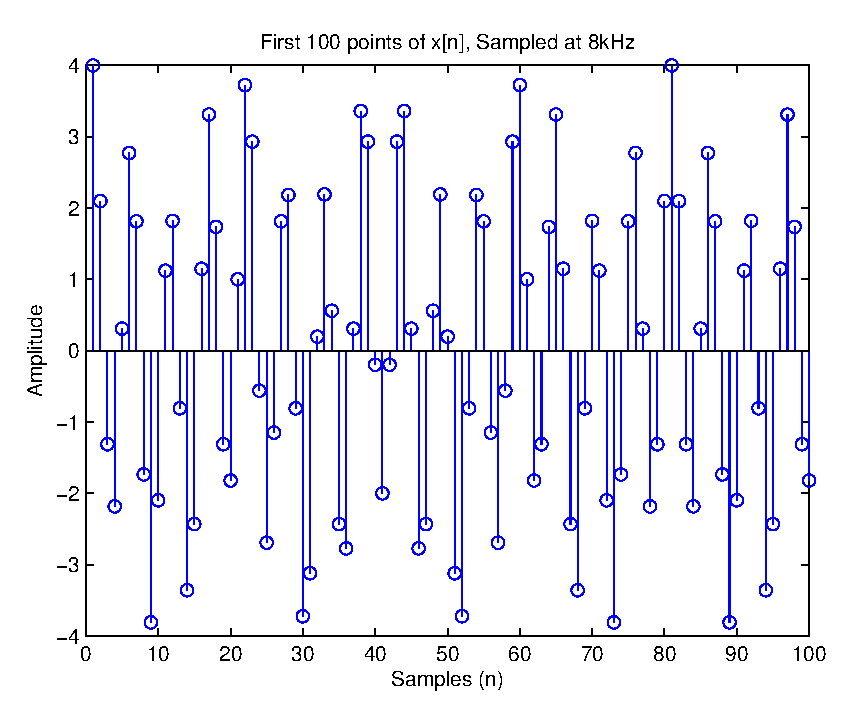
\includegraphics [width=4in]{Project3_03.eps}
		\caption{}
		\label{fig:}
	\end{center}
\end{figure}

% end of cell

    
           
        \subsection*{Part C}
    Plot the DTFT magnitude.The plot of this signal is included in Figure ~\ref{fig:figure4}.  An additional plot with the three repeated copies of the spectrum is included in Figure ~\ref{fig:figure5}.
\begin{lstlisting}[language=matlab]
figure(4);
plot([-4000:3999]/8000,fftshift(abs(fft(xn1(1:8000)))));
xlabel('Normalized frequency (\times 2\pi to give rad/sample)');

figure(5);
plot([-12000:11999]/8000,repmat(fftshift(abs(fft(xn1(1:8000)))),[1 3]));
xlabel('Normalized frequency (\times 2\pi to give rad/sample)');
\end{lstlisting}

\begin{figure}[here]
	\begin{center}
		\includegraphics [width=4in]{Project3_04.eps}
		\caption{}
		\label{fig:}
	\end{center}
\end{figure}

\begin{figure}[here]
	\begin{center}
		\includegraphics [width=4in]{Project3_05.eps}
		\caption{}
		\label{fig:}
	\end{center}
\end{figure}

% end of cell

    
           
        \subsection*{Part D}
    Does aliasing occur? Explain.Aliasing does not occur in this sampled signal.  The reason is that the sample rate is still above the Nyquist rate of 6000 kHz.  Below that threshold is where aliasing will start to occur.
% end of cell

    
           
        \subsection*{Question 3}
    Now consider a different sampling rate:
% end of cell

    
           
        \subsection*{Part A}
    Sample the waveform in \#1 at a sampling frequency of 2kHz for one second.
\begin{lstlisting}[language=matlab]
tsampled = [0:1/2000:1];
xn2 = 3*cos(3000*pi*tsampled) + cos(800*pi*tsampled);
\end{lstlisting}

% end of cell

    
           
        \subsection*{Part B}
    Determine how to plot the DTFT magnitude in Question 2, Part CThe DTFT magnitude plot is included in ~\ref{fig:figure7}. The additional plot with the three repeated copies of the spectrum is included in Figure ~\ref{fig:figure8}
\begin{lstlisting}[language=matlab]
figure(6);
stem(xn2(1:100));
title('First 100 points of x[n], Sampled at 2kHz');
xlabel('Samples (n)'); ylabel('Amplitude');

figure(7);
plot([-1000:999]/2000,fftshift(abs(fft(xn2(1:2000)))));
xlabel('Normalized frequency (\times 2\pi to give rad/sample)');

figure(8);
plot([-3000:2999]/2000,repmat(fftshift(abs(fft(xn2(1:2000)))),[1 3]));
xlabel('Normalized frequency (\times 2\pi to give rad/sample)');
\end{lstlisting}

\begin{figure}[here]
	\begin{center}
		\includegraphics [width=4in]{Project3_06.eps}
		\caption{}
		\label{fig:}
	\end{center}
\end{figure}

\begin{figure}[here]
	\begin{center}
		\includegraphics [width=4in]{Project3_07.eps}
		\caption{}
		\label{fig:}
	\end{center}
\end{figure}

\begin{figure}[here]
	\begin{center}
		\includegraphics [width=4in]{Project3_08.eps}
		\caption{}
		\label{fig:}
	\end{center}
\end{figure}

% end of cell

    
           
        \subsection*{Part C}
    Explain the differences between this plot and the one in \#2 based on the properties of sampling.The plot for the lower sampling frequency in Figure ~\ref{fig:figure7} has different values of magnitude than the plot for the higher sampling frequency in Figure ~\ref{fig:figure4}.  This means that some of the information about the original signal has been lost over the course of sampling it at the lower frequency.  Also, the frequencies have changed their positions due to undersampling.
% end of cell

    
           
        \subsection*{Part D}
    Does aliasing occur? Explain.Aliasing does occur in this sampled signal.  The reason is that the sampling rate has dropped below the Nyquist rate of 6kHz for the original signal.  It is immedeately apparant from the Fourier plot that the frequency spectrum is no longer close to the original.
% end of cell

    
           
        \subsection*{Question 4}
    We will now attempt to reconstruct the signal in \#1 from the sequence in \#2 using zero-order hold.
% end of cell

    
           
        \subsection*{Part A}
    Form a zero-order hold signal with 2 equal output samples per input sample.  Plot the first 100 points considered as a continuous-time signal.Using some MATLAB magic (reshape and repmat), I can do this without any loops
\begin{lstlisting}[language=matlab]
xn1_zoh=reshape(repmat(xn1',1,2)', length(xn1(:,1)), 2*length(xn1(1,: )));
figure(9);
plot(t(1:100),xn1_zoh(1:100));
xlabel('Time in Seconds'); ylabel('Amplitude');
title('First 100 Points of Waveform XN1 with Zero-Order Hold');
\end{lstlisting}

\begin{figure}[here]
	\begin{center}
		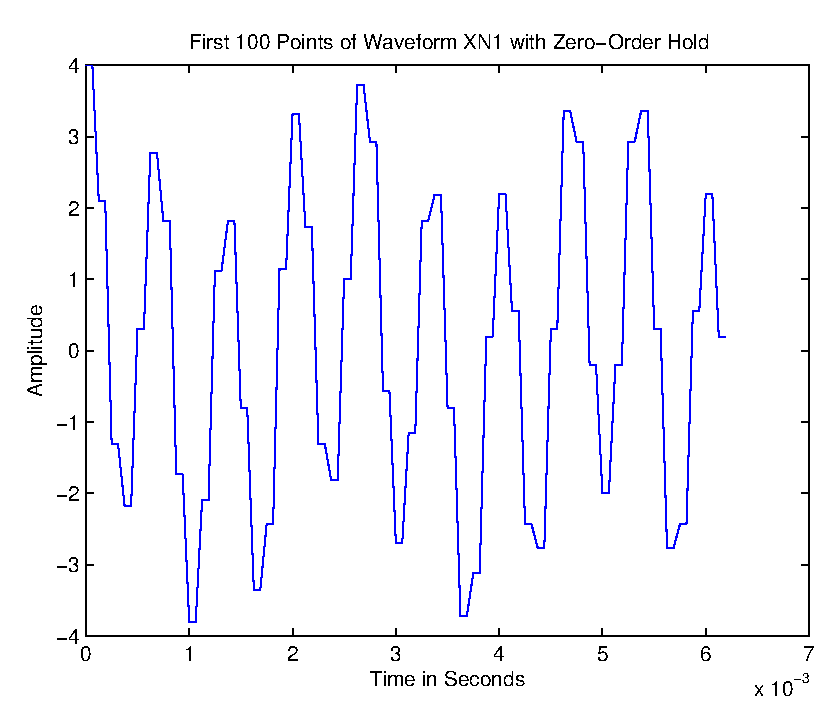
\includegraphics [width=4in]{Project3_09.eps}
		\caption{}
		\label{fig:}
	\end{center}
\end{figure}

% end of cell

    
           
        \subsection*{Part B}
    Plot the FT magnitude using the syntax from \#1, and explain what you observe.The Fourier transform plot included in Figure ~\ref{fig:figure10} now has some higher frequency components added from the zero-order hold.  These additional frequency components come from the "sharp" squared-off edges, which contain high-frequencies.
\begin{lstlisting}[language=matlab]
figure(10);
plot([-8000:7999],fftshift(abs(fft(xn1_zoh(1:2*8000)))));
xlabel('Normalized Frequency (\times 2\pi to give rad/s)');
title('Fourier-transform magnitude of waveform XN1 with ZOH');
\end{lstlisting}

\begin{figure}[here]
	\begin{center}
		\includegraphics [width=4in]{Project3_10.eps}
		\caption{}
		\label{fig:}
	\end{center}
\end{figure}

% end of cell

    
           
        \subsection*{Part C}
    Lowpass filter the ZOH signal as follows:
\begin{lstlisting}[language=matlab]
h = fir1(9,1/2);
xn1_reconstructed = filter(h,1,xn1_zoh);
\end{lstlisting}

% end of cell

    
           
        \subsection*{Part D}
    Plot the first 100 points considered as a continuous-time signal.The reconstructed continuous-time signal is included in Figure ~\ref{fig:figure11}
\begin{lstlisting}[language=matlab]
figure(11);
plot(t(1:100),xn1_reconstructed(1:100));
xlabel('Time in Seconds'); ylabel('Amplitude');
title('First 100 Points of Reconstructed Signal');
\end{lstlisting}

\begin{figure}[here]
	\begin{center}
		\includegraphics [width=4in]{Project3_11.eps}
		\caption{}
		\label{fig:}
	\end{center}
\end{figure}

% end of cell

    
           
        \subsection*{Part E}
    Plot the FT magnitude of the result using the syntax from \#1.  Explain what you observe. Is the signal in \#1 perfectly reconstructed? Justify your answer.The Fourier transform magnitude plots for the two signals are identical, so this leads me to believe that the signal has been perfectly reconstructed. This does not necessarily imply that the two signals are sample-for-sample identical, as can be seen in the differences between the continuous-time plots in Figure ~\ref{fig:figure11} and Figure ~\ref{fig:figure2}, but that the frequency content of both signals matches in both frequency and magnitude.
\begin{lstlisting}[language=matlab]
figure(12);
plot([-8000:7999],fftshift(abs(fft(xn1_reconstructed(1:2*8000)))));
xlabel('Normalized Frequency (\times 2\pi to give rad/s)');
title('Fourier-transform magnitude of reconstructed waveform');
\end{lstlisting}

\begin{figure}[here]
	\begin{center}
		\includegraphics [width=4in]{Project3_12.eps}
		\caption{}
		\label{fig:}
	\end{center}
\end{figure}

% end of cell

    
           
        \subsection*{Question 5}
    Play the sound from \#1, the ZOH sound, and the reconstructed sound using: soundsc(x,16000) Note any differences in the sounds.The first sound (original signal) was a mixture of two tones with nothing remarkable about it.  The second sound (ZOH) had some higher pitched ringing or noise in it. The higher pitched noise corresponds to what the Fourier transform magnitude plot in Figure ~\ref{fig:figure10}.  The third sound was similar to the first one.
\begin{lstlisting}[language=matlab]
% Commented so that I don't have to hear them every time I run the file.
% soundsc(xc,16000)
% soundsc(xn1_zoh,16000)
% soundsc(xn1_reconstructed,16000)
\end{lstlisting}

% end of cell

    
           
        \subsection*{Question 6}
    Reconstruct the signal in \#1 from the sequence in \#2 using linear interpolation.  You must use the filter function to get maximum credit. Compare the FT magnitude to the ZOH interpolation and the original. Explain the differences.The first step in linear interpolation is the upsampling of the signal. In this case, I upsampled by a value of 2 (made every other sample a zero after expanding the signal).The linear interpolation of the signal uses a filter with the following difference equation:$$y[n] = x[n] + \frac{1}{2}(x[n-1] + x[n+1]$$Which then expands to:$$y[n] = \frac{1}{2}x[n+1] + x[n] + \frac{1}{2}x[n-1]$$This is a non-causal filter (which uses a sample from a future reading). To get around this, I can use the padding options of the MATLAB filter command.To do this, I create the filter vector as I normally would, and MATLAB interprets this as:$$y[n] = \frac{1}{2}x[n] + x[n-1] + \frac{1}{2}x[n-2]$$Taking advantage of the initial conditions of the filter command, I made xn(2) and xn(1) initial conditions of the filter.  I have included a small proof of concept of this operation for the series [1,5] with an interpolation factor of 2.The Fourier transform magnitude of the linearly-interpolated waveform is included in Figure ~\ref{fig:figure13}.  Comparing this to Figure ~\ref{fig:figure10}, some of the same higher-frequency components are there, but at a much lower magnitude.  Doing the linear interpolation is similar to creating a low-pass filter as it "smooths off" some of the harsher transitions that the zero-order hold creates.
\begin{lstlisting}[language=matlab]
b = [.5 1 .5];

% Small proof of concept.
x = [1 0 -5 0 2 0 6 0 7 0];
x_linear = [x(1),filter(b,1,[x(3:end)],[.5*x(1),x(2)])]

xn1_upsampled = zeros(length(xn1)*2,1);
xn1_upsampled(1:2:length(xn1)*2) = xn1;

xn1_linear = [xn1_upsampled(1),...
    filter(b,1,xn1_upsampled(3:end),[.5*xn1(1),xn(2)])'];

figure(13);
plot([-8000:7999],fftshift(abs(fft(xn1_linear(1:2*8000)))));
xlabel('Normalized Frequency (\times 2\pi to give rad/s)');
title('Fourier-transform magnitude of linear interpolated waveform');
\end{lstlisting}

   {\color{lightgray} \small\begin{verbatim}
x_linear =

  Columns 1 through 5

    1.0000   -2.0000   -5.0000   -1.5000    2.0000

  Columns 6 through 9

    4.0000    6.0000    6.5000    7.0000

\end{verbatim} }

\begin{figure}[here]
	\begin{center}
		\includegraphics [width=4in]{Project3_13.eps}
		\caption{}
		\label{fig:}
	\end{center}
\end{figure}

% end of cell

    

\end{document}

